\begin{frame}{$\tau$ formulation of Full Approximation Scheme (FAS)}
  \begin{itemize}
  \item classical formulation: ``coarse grid \emph{accelerates} fine grid solution''
  \item $\tau$ formulation: ``fine grid improves accuracy of coarse grid''
  \item To solve $N u = f$, recursively apply
    \begin{equation*}
      \begin{split}
        \text{pre-smooth} \:\: & \quad \tilde u^h \gets S^h_{\text{pre}}(u^h_0, f^h) \\
        \text{solve coarse problem for $u^H$} \:\: & \quad N^H u^H = f^H + \underbrace{N^H \hat I_h^H \tilde u^h - I_h^H N^h \tilde u^h}_{\tau_h^H} \\
        \text{correction and post-smooth} \:\: & \quad u^h \gets S^h_{\text{post}} \Big( \tilde u^h + I_H^h (u^H - \hat I_h^H \tilde u^h), f^h \Big) \\
      \end{split}
    \end{equation*}
    \begin{tabular}{ll}
      \toprule
      $I_h^H$ & residual restriction \\
      $\hat I_h^H$ & solution restriction \\
      $I_H^h$ & solution interpolation \\
      $f^H = I_h^H f^h$ & restriction of forcing term \\
      $\{S^h_{\text{pre}},S^h_{\text{post}}\}$ & smoothing operations on the fine grid \\
      \bottomrule
    \end{tabular}
  \end{itemize}
\end{frame}

\begin{frame}{Multiscale compression and recovery using $\tau$}
  % \begin{tikzpicture}
  %   [>=stealth,
  %   every node/.style={inner sep=2pt},
  %   restrict/.style={thick,double},
  %   prolong/.style={thick,double},
  %   cprestrict/.style={green!50!black,thick,double,dashed},
  %   control/.style={rectangle,red!40!black,draw=red!40!black,thick},
  %   mglevel/.style={rounded rectangle,draw=blue!50!black,fill=blue!20,thick,minimum size=4mm},
  %   checkpoint/.style={rectangle,draw=green!50!black,fill=green!20,thick,minimum size=4mm},
  %   mglevelhide/.style={rounded rectangle,draw=gray!50!black,fill=gray!20,thick,minimum size=4mm},
  %   tau/.style={text=red!50!black,draw=red!50!black,fill=red!10,inner sep=1pt}
  %   ]
  %   \begin{scope}\scriptsize
  %     \newcommand\mgdx{2.1em}
  %     \newcommand\mgdy{1.9em}
  %     \newcommand\mgloc[4]{(#1 + #4*\mgdx*#3,#2 + \mgdy*#3)}
  %     \node[mglevel] (fine0) at \mgloc{0}{0}{4}{-1} {\mglevelfine};
  %     \node[mglevel] (finem1down0) at \mgloc{0}{0}{3}{-1} {};
  %     \node[mglevel] (cp1down0) at \mgloc{0}{0}{2}{-1} {$\mglevelcp+1$};
  %     \node[mglevel] (cpdown0) at \mgloc{0}{0}{1}{-1} {\mglevelcp};
  %     \node[mglevel] (coarser0) at \mgloc{0}{0}{0}{0} {\ldots};

  %     \node[mglevelhide] (cpup0) at \mgloc{0}{0}{1}{1} {};
  %     \node (cp1up0) at \mgloc{0}{0}{2}{1} {};

  %     \node (cpdown1) at \mgloc{4em}{0}{1}{-1} {};
  %     \node[mglevelhide] (coarser1) at \mgloc{4em}{0}{0}{1} {\ldots};
  %     \node[mglevel] (cpup1) at \mgloc{4em}{0}{1}{1} {\mglevelcp};
  %     \node[mglevel] (cp1up1) at \mgloc{4em}{0}{2}{1} {$\mglevelcp+1$};
  %     \node[mglevel] (finem1up1) at \mgloc{4em}{0}{3}{1} {};
  %     \node[mglevel] (fine1) at \mgloc{4em}{0}{4}{1} {\mglevelfine};

  %     \draw[->,restrict,dashed] (fine0) -- (finem1down0);
  %     \draw[->,restrict] (finem1down0) -- (cp1down0);
  %     \draw[->,restrict] (cp1down0) -- (cpdown0);
  %     \draw[->,restrict,dashed] (cpdown0) -- (coarser0);
  %     \draw[->,prolong,dashed] (coarser0) -- (cpup0);
  %     \draw[->,prolong,dashed] (cpup0) -- (cp1up0);

  %     \draw[->,restrict,dashed] (cpdown1) -- (coarser1);
  %     \draw[->,prolong,dashed] (coarser1) -- (cpup1);
  %     \draw[->,prolong] (cpup1) -- (cp1up1);
  %     \draw[->,prolong] (cp1up1) -- (finem1up1);
  %     \draw[->,prolong,dashed] (finem1up1) -- (fine1);

  %     \node[checkpoint] at (4em + \mgdx*4,\mgdy) (cp) {CP};
  %     \draw[>->,cprestrict] (fine1) -- node[below,sloped] {Restrict} (cp);

  %     \node[left=\mgdx of fine0] (bnanchor) {};
  %     \node[control,fill=red!20] at (1.1*\mgdx,3*\mgdy) {Solve $F(u^n;b^n) = 0$};
  %     \node[mglevel,right=of fine1] (finedt) {next solve};
  %     \draw[->, >=stealth, control] (fine1) to[out=20,in=170] node[above] {$b^{n+1}(u^n,b^n)$} (finedt);
  %     \draw[->, >=stealth, control] (bnanchor) to[out=45,in=155] node[above] {$b^n$} (fine0);

  %     % Recovery process
  %     \begin{scope}[xshift=7*\mgdx]
  %       \node[checkpoint] (rcp) at \mgloc{0}{0}{0}{0} {CP};
  %       \node[mglevel] (r0a) at \mgloc{0}{\mgdy}{0}{0} {CR};
  %       \node[mglevel] (r1a) at \mgloc{0}{\mgdy}{1}{1} {};
  %       \node[mglevel] (r0b) at \mgloc{2*\mgdx}{\mgdy}{0}{0} {CR};
  %       \node[mglevel] (r1b) at \mgloc{2*\mgdx}{\mgdy}{1}{1} {};
  %       \node[mglevel] (r2b) at \mgloc{2*\mgdx}{\mgdy}{2}{1} {\mglevelfine};
  %       \node[mglevel] (r1c) at \mgloc{6*\mgdx}{\mgdy}{1}{-1} {};
  %       \node[mglevel] (r0d) at \mgloc{6*\mgdx}{\mgdy}{0}{0} {CR};
  %       \node[mglevel] (r1d) at \mgloc{6*\mgdx}{\mgdy}{1}{1} {};
  %       \node[mglevel] (r2d) at \mgloc{6*\mgdx}{\mgdy}{2}{1} {\mglevelfine};

  %       \draw[-,prolong,green!50!black] (rcp) -- (r0a);
  %       \draw[->,prolong] (r0a) -- (r1a);
  %       \draw[->,restrict] (r1a) -- (r0b);
  %       \draw[->,restrict] (r0b) -- (r1b);
  %       \draw[->,restrict,dashed] (r1b) -- (r2b);
  %       \draw[->,restrict,dashed] (r2b) -- (r1c);
  %       \draw[->,restrict] (r1c) -- (r0d);
  %       \draw[->,restrict] (r0d) -- (r1d);
  %       \draw[->,restrict,dashed] (r1d) -- (r2d);

  %       \foreach \smooth in {finem1down0, cp1down0, cpdown0, coarser0,
  %         cpup1, cp1up1, finem1up1,
  %         r0b,r1c,r0d,r1d} {
  %         \node[above left=-5pt of \smooth.west,tau] {$\tau$};
  %       }
  %       \node[rectangle,fill=none,draw=green!50!black,thick,fit=(rcp)(r2d)] (recoverbox) {};
  %       \node[rectangle,draw=green!50!black,fill=green!20,thick,minimum size=6mm,above={0cm of recoverbox.south east},anchor=south east] (recover) {FMG Recovery};
  %     \end{scope}
  %     \node (notation) at (-7.5*\mgdx,2*\mgdy) {
  %       \tiny
  %       \begin{minipage}{22em}\raggedright \sf
  %         $\bullet$ checkpoint converged coarse state \\
  %         $\bullet$ recover using FMG anchored at $\mglevelcp+1$ \\
  %         $\bullet$ compatible relaxation (CR) as coarse solve \\
  %         $\bullet$ $\tau$ correction is local, only $\mglevelcp$ neighbor points \\
  %         $\bullet$ survivors continue MG cycles with stale $\tau$
  %       \end{minipage}
  %     };
  %   \end{scope}
  % \end{tikzpicture}
  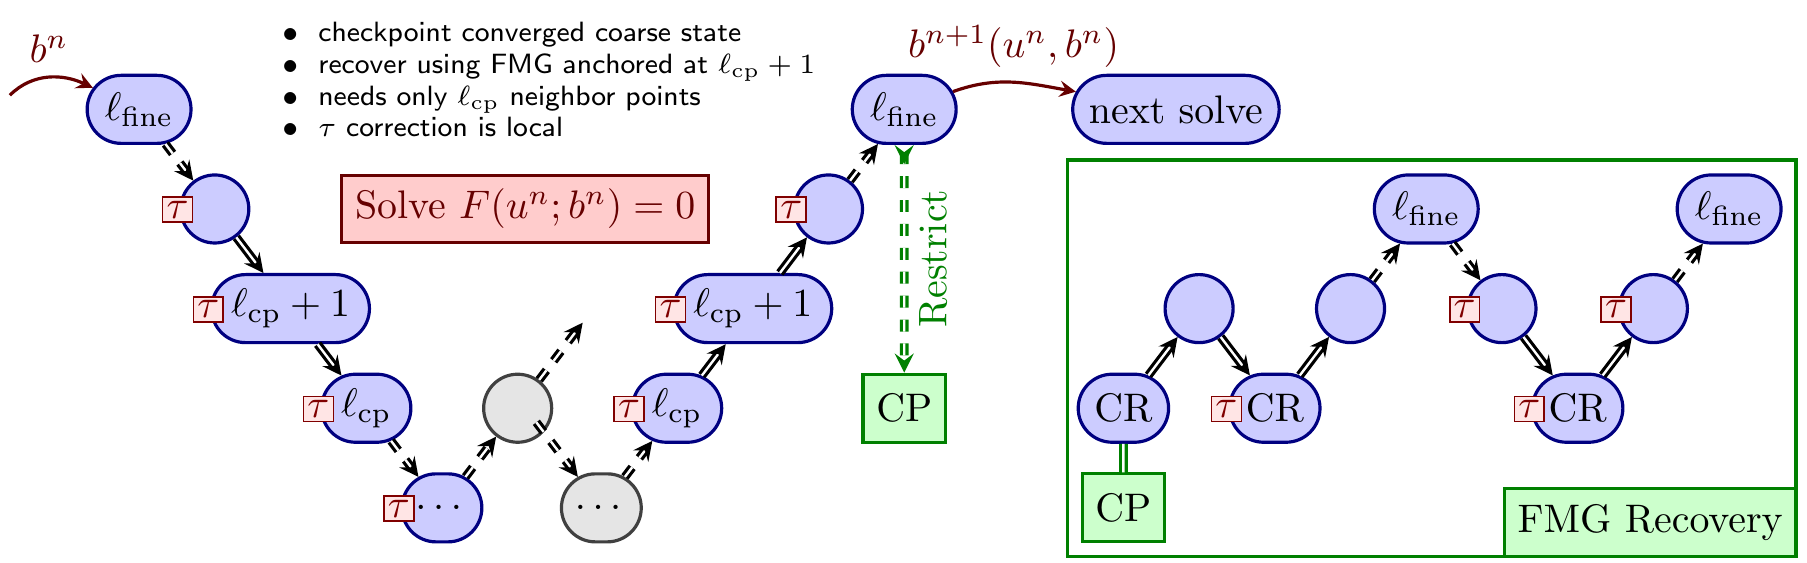
\includegraphics[width=\textwidth]{FMGRecovery}
    \begin{itemize}
    \item Compress transient simulation with local decompression
    \item Remove communication from all but coarse grid
      \begin{itemize}
      \item Convergence speed not affected, modest redundant computation
      \end{itemize}
    \item In-situ visualization and reanalysis with very few full checkpoints
    \item Checkpointing for discrete adjoints
    \item Resiliency to hardware failure
    \end{itemize}
\end{frame}
